In Personal Informatics people collect different kinds of personal data voluntarily for the purpose of self-reflection and gaining knowledge about themselves \cite{Li2010}. Personal Informatics have identified various aspects of self-tracking activities \cite{Li2010} and since self-tracking is a common denominator to the fields of both telehealth and Personal Informatics we (in the absence of technology knowledge in telehealth) used the literature of Personal Informatics as an analytical lens for the field of telehealth. 

\begin{figure}[!h] \centering
			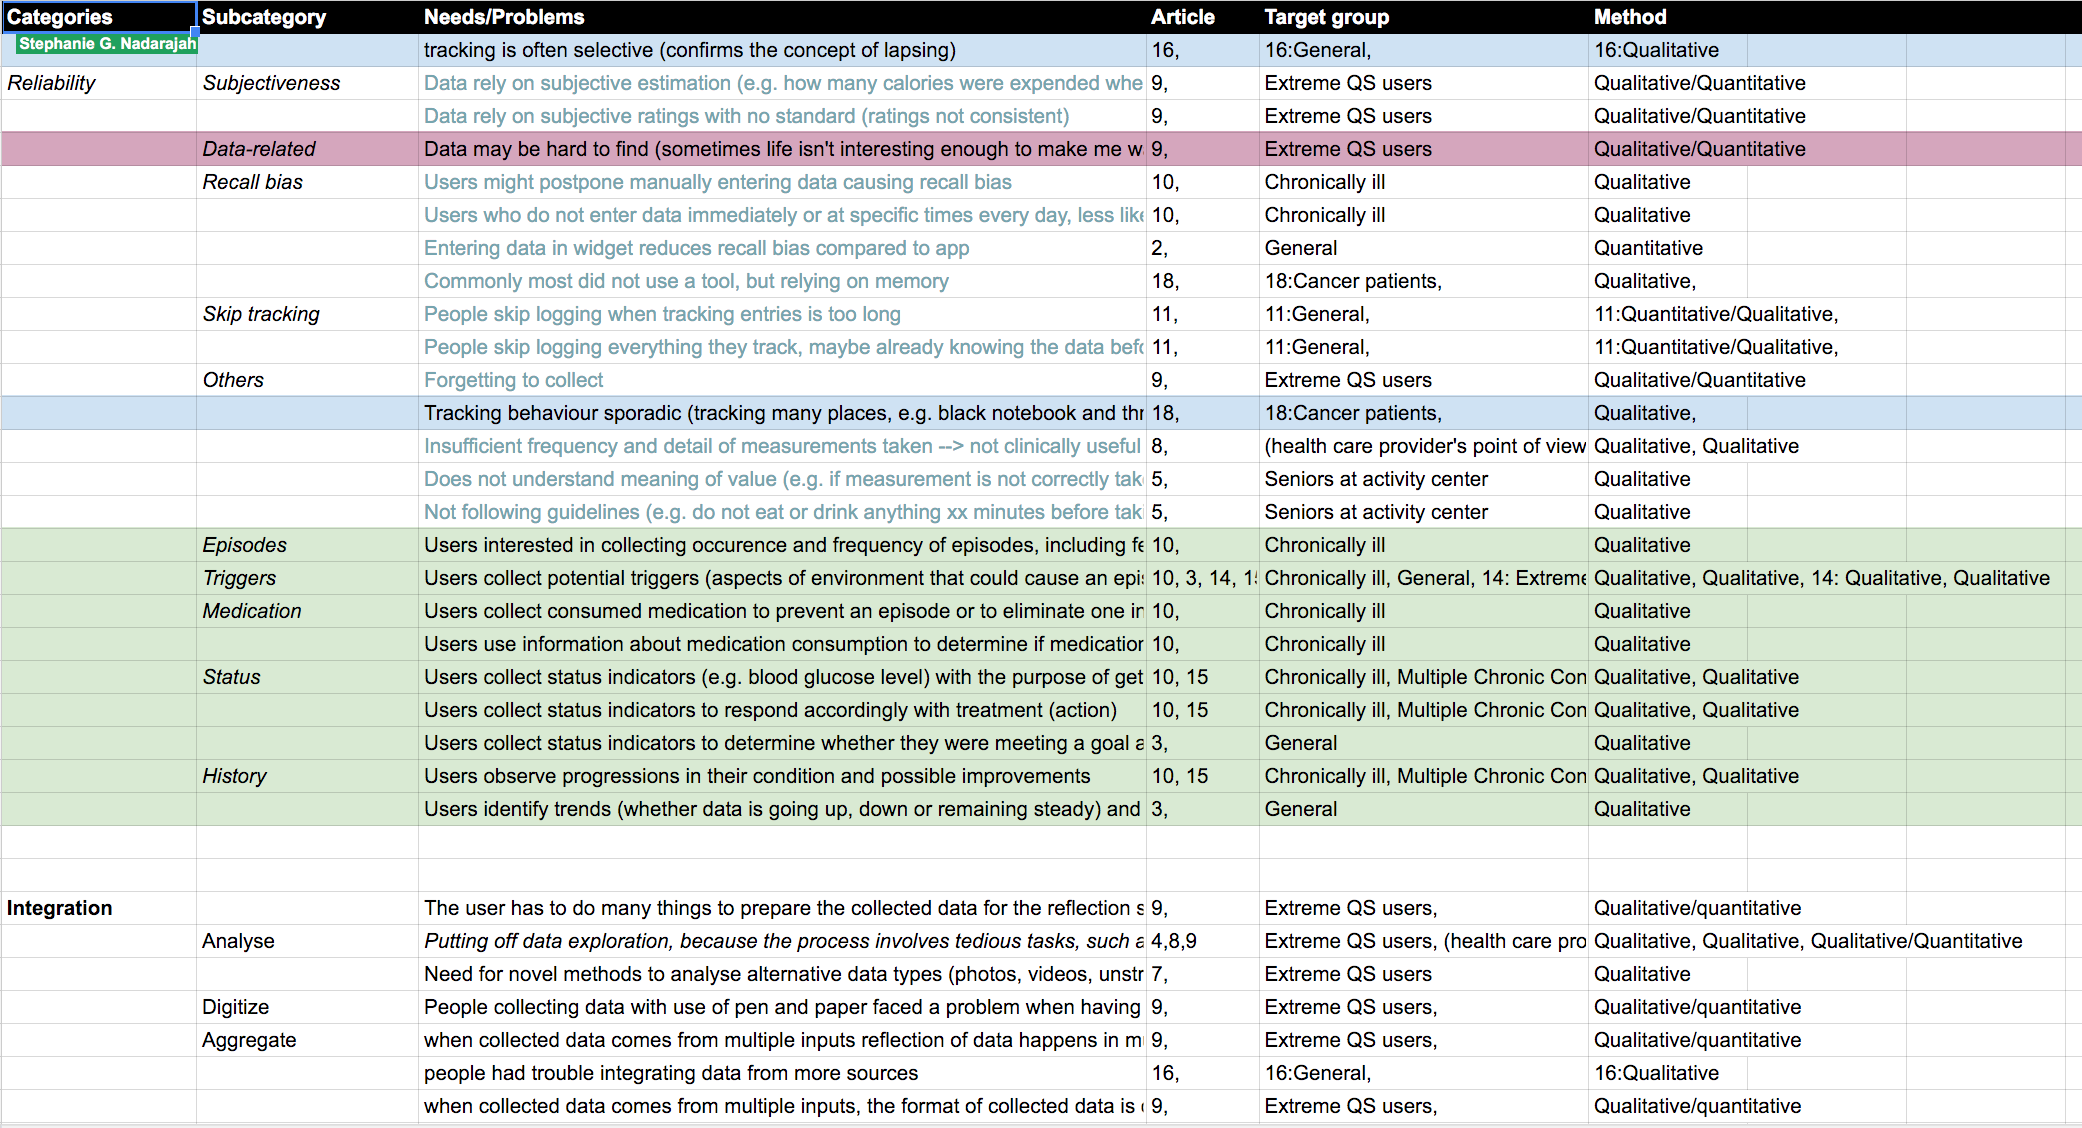
\includegraphics[width=1\textwidth]{Images/PI/researchtable.png}
		\caption{Research table with user needs identified in Personal Informatics literature} \label{fig:PI}
\end{figure}

We analysed the literature of Personal Informatics for different drivers for self-tracking, how people track and the barriers that typical arise in self-tracking activities (See Figure \ref{fig:PI}). We distinguish between self-tracking that is initiated by oneself (henceforth referred to as discretionary tracking) and self-tracking initiated by a healthcare provider (henceforth referred to as prescribed tracking). While discretionary trackers take up self-tracking voluntarily, prescribed trackers are either recommended or required to track by a healthcare provider (i.e. a physician or a nurse), e.g. for a specific treatment, for long-term performance or approval for surgery. 

\section{Why People Track} 
From the literature, we classified main motivations for self-tracking into five categories.

\paragraph{Documentation}
Some discretionary trackers are mainly interested in documenting their activities, rather than changing them \citep{Rooksby2014}. Self-tracking not for one's own purpose, but partly or largely to create records for the healthcare providers was a reason for imposed self-tracking in \citep{Ancker2015}. 

\paragraph{Life Experience} 
People tracking for life experience are mainly discretionary trackers who track out of natural curiosity about what their data might reveal about themselves \citep{Li2010, Epstein2015} or because of an interest in quantitative data \citep{Li2010, Rooksby2014}. Others aim to discover new tools or because of an interest in gadgets and technology \citep{Li2010, Rooksby2014}. 

\paragraph{Communication} 
Discretionary trackers tracking for documentation also used the data as a way of underscoring their effort through sharing, e.g. using a pedometer to convince a friend that they walked a lot \citep{Rooksby2014}. Others used it for direct social benefits (for practical reasons e.g. informing others about their location, for social engagement, etc. \citep{Epstein2015}) and in response to gamification incentives, such as to score points or achievements \citep{Rooksby2014}. Some self-trackers use tracked data as evidence when they find empathy of healthcare providers lacking, or in order to show a complete picture of their life, when they do not find measurements taken in the clinic sufficient \citep{Chung2016}. Some hope that self-tracking can help communicate their condition to family members \citep{MacLeod2014}. 

\paragraph{Self-Knowledge} \label{selfknowledge}
Self-trackers in this category track to get a sense of the current state of their condition \citep{MacLeod2014, Ancker2015}. Some are motivated to track in order to identify potential links between different factors, e.g. tracking medication and diet to identify what caused stomach problems \citep{Rooksby2014}. They also self-track in order to learn what to add in their lives, in order to prevent undesirable health-related episodes (e.g. initiating medication to prevent a worsening of condition) or what to remove in order to reduce impact of such episodes (e.g. stop smoking to reduce symptom severity) \citep{MacLeod2014}. These motives indicate that this type of self-trackers are also partially motivated to self-improve. 

\paragraph{Self-Improvement} \label{selfimprove}
Common to these self-trackers is a desire to change or maintain a behaviour in order to improve their well-being or lifestyle \citep{MacLeod2014, Ancker2015, Chung2016, Li2011, Whooley2014}. Self-trackers in this category are goal-driven (e.g. have the goals "avoid drinking coffee X hours before sleeping" or "run three times a week") and regulate their progress towards their goal \citep{Chung2016, Rooksby2014, Li2011}. MacLeod et al. found that prescribed self-trackers were motivated due to the resulting self-efficacy and sense of agency. Tracking made them feel they were helping managing their condition and empowered to take control of their own health. Despite being initiated to self-track by their provider, a majority of the self-trackers were motivated to continue self-tracking even after their provider did not require it anymore \citep{MacLeod2014}. 

\section{How People Track}
Researchers have proposed different models for understanding, how self-trackers concretely use personal informatics systems over time. Li et al. proposed a five-staged model describing, how self-trackers transition between these stages: (1) \textit{preparation} (user determines what and how to track data), (2) \textit{collection} (user tracks data), (3) \textit{integration} (user prepares data for reflection), (4) \textit{reflection} (user explores data to gain self-knowledge) and (5) \textit{action} (user decides what to do with newfound self-knowledge) \citep{Li2010}. The \textit{reflection} stage can further be divided into \textit{maintenance} and \textit{discovery} \citep{Li2011}. Opposed to the \textit{maintenance} phase, self-trackers in the \textit{discovery} phase do either not know their goal and/or have not identified important factors yet to determine appropriate actions \citep{Li2011}. 

Epstein et al. divided the \textit{preparation} stage into \textit{deciding} and \textit{selecting}. Self-trackers first decide to track and then select a tool to support their self-tracking efforts \citep{Epstein2015}. Li et al. describe the five-staged model as linear \citep{Li2010}, whereas Epstein et al. further describe \textit{tracking} and \textit{acting} as ongoing processes of collecting, integrating and reflecting. Epstein et al. do not separate collecting, integrating and reflecting into stages as these activities can and do occur simultaneously \citep{Epstein2015, MacLeod2014}. Epstein et al.'s model was developed using almost the same methods as Li et al. though (according to the authors) conducted on a more general population (recruited from an online crowdsourcing marketplace) \citep{Epstein2015}. The \textit{integration} stage can be more or less apparent to the self-tracker depending on type of personal informatics system. Both Whooley et al. and Li et al. write about two types; system-driven and user-driven. In a user-driven personal informatics system the self-tracker is responsible for the activities involved (e.g. aggregating and analysing data) in contrast to system-driven personal informatics system where the system is responsible of the activities, thus requiring less effort of the self-tracker \citep{Whooley2014,Li2010}. Epstein et al. further included stages of \textit{lapsing} and \textit{resuming} into their model, accounting for users sometimes stopping to track for either longer or shorter periods (for instance because of forgetting to track and skipping maybe already known data) and the opportunity of resuming tracking later \citep{Epstein2015}. The nature of lapsing and resuming during self-tracking was also confirmed by \citep{Rooksby2014}. 

We use Epstein et al.'s model as a lens to discuss our own findings on user needs and concerns in the following section. 

\subsection{Deciding and Selecting}
\paragraph{Preparation}
In the \textit{preparation} stage, people decide what to track and how they want to track. One common problem people experience is not always knowing what to track or what questions to ask \citep{Li2011, Choe2014, Chung2015, Patel2012}. Discretionary trackers might not have identified what goals they are trying to meet and/or might not have identified what factors influence their behaviour (\textit{discovery} phase). This means that after an initial phase of tracking, they might have to redefine what to track and what questions to ask \citep{Choe2014}. This mirrors  Li et al.'s findings on self-trackers tending to transition between the \textit{maintenance} and \textit{discovery} phase \citep{Li2011}. 

Prescribed trackers experience that healthcare providers recommend symptom tracking, but sometimes give little support on what to track and how to track (e.g. frequency of tracking) \citep{Patel2012}. Some health conditions involve many symptoms that sometimes arise unexpectedly. Patel et al. found that patients who experienced symptoms that providers had not suggested tracking, had to figure out themselves, whether these symptoms were important and if additional tracking was needed \citep{Patel2012}. Tracking the wrong data or not tracking well enough to gain benefits can according to healthcare providers lead to loss of motivation to keep tracking \citep{Chung2015}.  

Both Patel et al. and Chung et al. found that tools recommended for self-tracking by healthcare providers did not always meet the needs of the self-trackers e.g. tracking symptoms self-trackers want to track \citep{Patel2012, Chung2016}. As a result, self-trackers found other tools or designed their own tracking systems, such as notebooks, health diaries and specific applications. If these tools did not support collaborative review or other requirements from the healthcare provider, it sometimes created tension between patients and providers later in the \textit{reflection} stage \citep{Chung2016}. 

\subsection{Tracking and Acting}					
\paragraph{Collection}
In the \textit{collection} stage self-trackers collect data about themselves. 

Even though self-trackers do not know how to track well or accurately enough \citep{Chung2015, Patel2012}, they develop their own systems for tracking. Prescribed trackers are only offered little support from health care providers, but do not know how to improve their systems. The self-developed systems are often cumbersome and incomplete and prescribed trackers who choose to track a breadth of health issues pose a significantly challenge on themselves \citep{Patel2012}. Self-tracking too many things can lead to tracking fatigue \citep{Choe2014}. 

Rooksby et al. questioned that people could or always wanted to do rational data collection \citep{Rooksby2014}, which leads to measures with low reliability. Self-trackers skipped tracking when data entries were too long or when data was known beforehand they did not always see the benefit of tracking it \citep{Epstein2015}. Self-trackers might also simply forget to track \citep{Li2010}. 

Prescribed self-trackers found tracking time consuming and requiring effort \citep{Ancker2015} hampering incorporation of tracking into daily routines \citep{Verdezoto2015, Ancker2015}. Self-trackers do not want to spend too much time on entering data \citep{Choe2013, Li2010}. This not only due to act of entering data but includes preparation to do so. For example, resting a number of minutes before taking blood pressure measures increased time and effort \citep{Verdezoto2015}. Incorporation difficulties lead to skipped primary tracking and secondary data, e.g, whether guidelines had been followed by  smoking before taking a blood pressure reading. This reduced reliability and difficulties in data interpretation \citep{Verdezoto2015}. Among prescribed self-trackers, measurements were found not to be clinically useful because of insufficient frequency and detail in tracking \citep{Chung2015}. 

Some subjective measurements also affect the reliability of the data. For instance, when a self-tracker subjectively quantifies expended calories when lifting weights or when self-trackers are required to subjectively assess without any standard (e.g. when wanting to rate relationship satisfaction and ratings are not consistent) \citep{Li2010}. \citep{piloting} suggests similar problems, where prescribed self-trackers subjectively assessed, whether they coughed more or experienced more dyspnea than usual. Some found it difficult to assess such questions, as they were constantly symptomatic and were in doubt of what standard they should compare them to. Data granularity impeded collection when self-trackers were overthinking, while trying to rate mood on a scale from 0 to 10 \citep{Oh2015}. 

Recall bias can reduce data reliability as prescribed trackers did not use a tool for tracking but relied on memory \citep{Patel2012} or postponed manually entering data \citep{MacLeod2014}. Self-trackers who do not enter data immediately or at specific times each day are less likely to remember making the tracking and they are also less confident in the accuracy of their own data \citep{MacLeod2014}. \citep{Li2010} found that one participant problematized the fact that s/he did not have ready access to her tracking device (a computer) at the time symptoms happened. Some prescribed self-trackers appreciate doing tracking in a notebook because of its portability even though it provides little structure \citep{MacLeod2014}. Patel et al. tried to improve the reliability of the data and decrease recall bias by developing a smartphone application enabling prescribed self-trackers to do manual realtime tracking with use of self check-ins for logging symptoms. According to their qualitative evaluation their app was successful but new user needs emerged \citep{Patel2012}. Prescribed self-trackers appreciate the ability to collect a variety of data \citep{MacLeod2014, Patel2012}, which is why prescribed self-trackers appreciate flexibility of notebooks \citep{MacLeod2014} and fortunately the smartphone application by Patel et al. supported prescribed self-trackers in tracking self-selected variables on a 0 to 4 scale, but some participants made a workaround to generate new units that were not initially supported, e.g. "took all pills". The authors report that their smartphone application was engaging, but it still required a great deal of effort for users to track. They end up recommending further simplification within tracking for instance by voice commands \citep{Patel2012}. Another study tried to simplify tracking with use of an Android interactive widget, which allowed easy input of data. The widget was accompanied by an associated app in one condition and another condition, where they only had the app for inputting data. Participants in the condition utilized with the widget had a significantly higher adherence and they also captured an event significantly closer to its actual time than participants in the non-widget condition \citep{Choe2015}. 

\paragraph{Integration}
In this stage the personal data is "prepared combined and transformed for the user to reflect on" \citep{Li2010}, which involves data aggregation, data analysis, statistical tests and creation of data representations \citep{Li2010}. 

Self-trackers that collect data with pen and paper face a problem, because they have to transcribe data into an electronic format, in order to visualize their data. Self-trackers has to do many things in order to prepare the data for reflection \citep{Li2010}, but if the integration is system-driven less effort is required by the self-tracker \citep{Li2011, Whooley2014} making integration less apparent. There are different trade-offs in the integration stage, depending on whether the system is system-driven or user-driven. User-driven systems expect the user to be able to analyse the data and ascertain the best way of creating a representation, which is of interest to curiosity-driven self-trackers that want to integrate data manually and explore the novel insights that data can offer them. This is in contrast to outcome oriented self-trackers who know what they are looking for in the data, they strive at using automatic integration systems allowing them to concentrate on reflection. Self-trackers driven by self-improvement only manually integrate data when the system does not support them with their goals and when they are sufficiently motivated and skilled. The manual integration process is an iterative process of moving back and forth between representation creation and reflection \citep{Whooley2014}. 

Previous work shows that that data exploration is sometimes postponed, since it involves tedious tasks, such as cleaning up data, formatting and running statistical tests \citep{Choe2014, Chung2015, Li2010}. Rooksby et al. found that it is unrealistic to believe that self-trackers only act, when data has been validated and thoroughly analysed \citep{Rooksby}, while Choe et al. write that data interpretation is a key hurdle where self-trackers drown in information and a common barrier is self-trackers have poor skills in analysing data and creating (plus identifying) the most appropriate visualization \citep{Choe2014}. 

Whooley et al. found that self-trackers might create many different visual representations for exploration of the same data, especially if they are driven by curiosity \citep{Whooley2014}. 
Different types of visualization and data representations was identified by Whooley et al. where binary representations (distil data integrated into one of two results) and structured representations (tables and graphs, which show a relationship between two or more variables) are typically created by self-trackers that are driven by self-improvement \citep{Whooley2014}.

Problems arise when collected data comes from multiple inputs. In such cases \citep{Li2010} found that reflection happens in multiple outputs and it is not in a format for reflection. This found of barrier is in agreement with \citep{Rooksby2014}, who found that people had trouble integrating data from more inputs. Another study specifically reported that different tracking tools do not support the exploration of the data in one place. Tools further do not support data exportation making aggregation a challenge \citep{Li2011}. 

\paragraph{Reflection}
People explore collected data to gain self-knowledge and reflection already occurs while entering data \citep{Whooley2014, MacLeod2014, Epstein2015}. Regardless of whether self-trackers have a health-related condition or not, data collection can have strong emotional meaning \citep{Li2010, Ancker2015}. Data can remind people of negative aspects of e.g. an illness, which can be depressing or scary, causing people not wanting to track or review their data \citep{Ancker2015}. 

Experienced self-trackers become frustrated by mismatches between subjective feeling and objective measures (e.g. when a health-related quantitative value spikes without a clear reason or matching subjective assessment) \citep{Ancker2015}. These mismatches can reduce self-trackers' confidence that they understand and are capable of managing their disease. Some self-trackers resist their healthcare providers' interpretation but relying on their own identified "normal range", i.e. values that made them feel well \citep{Ancker2015}. Self-trackers with a health-related condition further preferred to interpret their data in light of their own personal and medical history and/or symptoms rather than striving for provider-recommended values. 

Another concern related to the language healthcare providers use, when they review data with the patients. Healthcare providers found that it was better to use non-judgmental language (e.g. high/low) rather than judgmental language (e.g. good/bad) about patients readings, in order to not discourage patients, who might think they are being judged \citep{Ancker2015}. 

Sometimes patients need to share their data with multiple healthcare providers for review \citep{Chung2016}. Some patients need support from providers in confirming their data interpretation, while others require expert assistance in understanding the meaning of numeric values \citep{Verdezoto2015}. For example, when taking blood pressure measures on a digital device, elderly initially needed assistance to understand the meaning of the numeric values. The provider had to explain that several readings were needed to compare and support their interpretation \citep{Verdezoto2015}. 

While discretionary trackers have difficulties interpreting large amounts of data \citep{Choe2014}, healthcare providers similarly sometimes struggle with interpreting data sets that include additional and not always relevant information \citep{Chung2015, Chung2016}. Even though providers suggested tracking a specific factor, some apps encouraged self-trackers to input other information and displayed unnecessary information that hindered effective review by time-constrained providers \citep{Chung2016}. Self-trackers sometimes also experienced not having collected enough data to observe trends (going up, down or remaining steady) and patterns \citep{Li2011} or that data collection has been too intermittent to allow for meaningful visual representations \citep{Li2010}. 

Self-trackers find visualizations helpful supporting them in understanding their data \citep{Choe2014}, but also experienced difficulties when visualization were overly technical or irrelevant to their interests. One self-tracker mentioned that she found the provided visualizations difficult to understand in relation to cutting her caffeine intake \citep{MacLeod2014}. The representation consisted of two types of visualizations: (1) A timeline based graph showing goals momentum by period (over a week) and (2) a histogram showing goal success by period (over a week). She liked visualization that were quickly and easily readable.

Sometimes self-trackers are interested in review data over long term to identify trends and patterns, but not all tools supports that. E.g. one participant might collect information about sleep quantity, but the interface might present only the numeric values, where a simple bar graph might have been more useful to review past history \citep{Li2011}. In the \textit{maintenance} phase self-trackers need to see trends, in order to assess progress towards their goal. Additionally, MacLeod et al. found that tools do not support comparing factors by giving users the ability to sort and filter data, supporting them in reflecting in ways meaningful for them \citep{MacLeod2014}.Self-trackers need tools to be flexible and allow for a holistic view of the collected data (e.g. showing information for several months at once), which was not always supported by tools with time filters \citep{Li2010}. Some self-trackers want to focus on some specific information of interest. \citep{Whooley2014} found that self-trackers with programming skills added interactivity to their tools in order to drill into information of interest.

\paragraph{Action}
People decide what action to take based on the findings from the reflection stage. Sometimes people do not have the necessary knowledge, in order to identify appropriate action and improve their data, either because they have collected the wrong data \citep{Choe2014, Chung2015} (e.g. collected food and symptoms, when it might be ingredients that trigger the symptoms) or because they are in need of more (expert) knowledge about their data and how it can be improved \citep{Verdezoto2015, Li2010, Oh2015}. 

Verdezoto \& Gr{\"o}nvall found that elderly interested in self-tracking were well aware of and understood if behaviour change was needed. But despite motivation to learn, they did not know what behavior change was needed to get better outcomes \citep{Verdezoto2015}, suggesting a need for actionable advice. Most systems do not help self-trackers in drawing actionable conclusions from the data \citep{Chung2015, Li2010}. Therefore self-trackers seek advice from their healthcare providers in case of having a health-related condition to manage \citep{Li2010}. 

\paragraph{Lapsing and Resuming}
Lapsing and resuming occur when a self-tracker temporarily stops tracking and later resumes. Some might even not resume, for instance when a self-tracker forget to track several times, the self-tracker may decide it is not worth the trouble \citep{Epstein2015}. 

Studies have found different reasons for lapsing aside from the abovementioned forget-related lapse. Rooksby et al.'s found from interviewing 22 people interested in activity tracking that several of them tracked everything they ate while others went through short periods of tracking revealing tracking as being selective to each self-tracker, which potentially can cause lapses \citep{Rooksby2014}. Epstein et al. found that lapses typical begins with barriers to collection. Lapsing can also be caused by barriers to integration or reflection. A self-tracker going on holiday is also a known reason for lapses as well as injuries or when life habits changes. Some also lapse tracking private things if the PI system emphasize sharing. When self-trackers already know the data they can decide not to track, especially when they do not see the benefit. Lapses can be provoked of different reasons depending on type of self-tracker. Curiosity-driven trackers lapse tracking when tracking tools often require maintenance (e.g. charging battery). Self-trackers driven by self-improvement lapse if collection becomes too much work \citep{Epstein2015}. 

After a long lapse (stopped tracking for months) self-trackers will sometimes instead of resuming start integrating or reflecting on data and eventually later decide whether to resume. In relation to resuming, it is today unknown how a PI system should react when someone decides to resume after a lapse, especially when the system archives discouraging past data \citep{Epstein2015}.